\documentclass[twoside]{article}
\usepackage{aistats2017}

% If your paper is accepted, change the options for the package
% aistats2015 as follows:
%
%\usepackage[accepted]{aistats2015}
%
% This option will print headings for the title of your paper and
% headings for the authors names, plus a copyright note at the end of
% the first column of the first page.

%%%%%%%%%%%%%%%%%%%%%%%%%%%%%%%%%%%%%%%%%%%%%%%%%%%%%%%%%%%%%%%%%%%%%%%%%%%%%%%%

\usepackage{amsmath}
\usepackage{amssymb}
\usepackage{amsthm}
\usepackage{mathtools}
\usepackage{graphicx}
\usepackage{rotating}
\usepackage{xcolor}
\usepackage[inline]{enumitem}

\usepackage{algorithm}
\usepackage[noend]{algpseudocode}
%\usepackage{algorithmicx}
%\usepackage{algorithm2e}

%\usepackage[authordate,bibencoding=auto,strict,backend=biber,natbib]{biblatex-chicago}
\usepackage[round]{natbib}   % omit 'round' option if you prefer square brackets
\bibliographystyle{plainnat}

\usepackage{tikz}
\usepackage{pgfplots}
\pgfplotsset{width=7cm,compat=1.8}

%%%%%%%%%%%%%%%%%%%%%%%%%%%%%%%%%%%%%%%%

\newtheorem{cor}{Corallary}
\newtheorem{theorem}{Theorem}
\newtheorem{lemma}{Lemma}
\newtheorem{assumption}{Condition}

\DeclareMathOperator*{\argmin}{arg\,min}
\DeclareMathOperator*{\argmax}{arg\,max}
\DeclareMathOperator*{\vecspan}{span}
\DeclareMathOperator*{\affspan}{aff}
\DeclareMathOperator*{\subG}{subG}
\DeclareMathOperator*{\tr}{tr}

\newcommand{\zero}{\text{\textbf{0}}}
\newcommand{\Zproj}{Z^{\textit{proj}}}
\newcommand{\Zreopt}{Z^{\textit{owa}}}
\newcommand{\nreopt}{n^{\textit{owa}}}
\newcommand{\Q}{\mathcal{Q}}
\newcommand{\Y}{\mathcal{Y}}
\newcommand{\X}{\mathcal{X}}
\newcommand{\W}{{\hat \Theta^{\textit{owa}}}}
\newcommand{\Wowa}{{\hat \Theta^{\textit{owa}}}}
\newcommand{\Waff}{\mathcal{\hat A}}
\newcommand{\WaffE}{{\mathcal{\hat A}_\E}}
\newcommand{\Wave}{{\mathcal{\hat W}^{ave}}}
\newcommand{\Wtave}{{\mathcal{W}^{ave,*}}}
\newcommand{\V}{\mathcal{V}}
\newcommand{\A}{\mathcal{A}}
\newcommand{\D}{\mathcal{D}}
\newcommand{\E}{\mathbb{E}}
\newcommand{\vv}{\mathbf{v}}
\newcommand{\x}{\mathbf{x}}
\newcommand{\y}{\mathbf{y}}
\newcommand{\w}{\theta}
\newcommand{\wkl}{\hat\w^{kl}}
\newcommand{\ahat}{\hat\alpha}
\newcommand{\afull}{\ahat^{\textit{full}}}
\newcommand{\wowa}{\hat\w^{owa}}
\newcommand{\wowafull}{\hat\w^{\textit{owa,full}}}
\newcommand{\wowastar}{\hat\w^{\textit{owa,*}}}
\newcommand{\wave}{\hat\w^{ave}}
\newcommand{\wtave}{\E\hat\w^{ave}}
\newcommand{\waver}{\hat\w^{ave,r}}
\newcommand{\wboot}{\hat\w^{boot}}
\newcommand{\wmle}{\hat\w^{mle}}
\newcommand{\wmler}{\hat\w^{mle,r}}
\newcommand{\wstar}{{\w^{*}}}
\newcommand{\wq}{\hat\w^{q}}
\newcommand{\wqstar}{\hat\w^{q^*}}
\newcommand{\dist}{\mathcal{D}}

\newcommand{\tbias}{t_{\text{\textit{bias}}}}
\newcommand{\tvar}{t_{\text{\textit{var}}}}

\newcommand{\I}{\mathcal I}
%\newcommand{\I^{-1}}{\I^{-1}}
\newcommand{\law}{\ensuremath{\xrightarrow{L}}}
\newcommand{\normal}[2]{\ensuremath{\mathcal{N}\left({{#1}},{{#2}}\right)}}
\newcommand{\subnormal}[1]{\ensuremath{\subG\left({{#1}}\right)}}
\newcommand{\trans}[1]{\ensuremath{{#1}^{\mathsf{T}}}}
\newcommand{\ltwo}[1]{{\lVert {#1} \rVert}}
\newcommand{\ltwobig}[1]{{\left\lVert {#1} \right\rVert}}
\newcommand{\lone}[1]{{\lVert {#1} \rVert}_1}
\newcommand{\lzero}[1]{{\lVert {#1} \rVert}_0}
\newcommand{\proj}[1]{\pi_{{#1}}}
\newcommand{\prob}[1]{\Pr\left[{#1}\right]}

\DeclarePairedDelimiterX{\infdivx}[2]{(}{)}{%
  #1\;\delimsize\|\;#2%
}
\newcommand{\kl}{\text{KL}\infdivx}

\newcommand{\ignore}[1]{}
\newcommand{\fixme}[1]{\textbf{FIXME:} {#1}}

%%%%%%%%%%%%%%%%%%%%%%%%%%%%%%%%%%%%%%%%%%%%%%%%%%%%%%%%%%%%%%%%%%%%%%%%%%%%%%%%

\begin{filecontents}{paper.bib}

@book{lehmann1999elements,
  title={Elements of large-sample theory},
  author={Lehmann, Erich Leo},
  year={1999},
  publisher={Springer Science \& Business Media}
}

@inproceedings{merugu2003privacy,
  title={Privacy-preserving distributed clustering using generative models},
  author={Merugu, Srujana and Ghosh, Joydeep},
  booktitle={Data Mining, 2003. ICDM 2003. Third IEEE International Conference on},
  pages={211--218},
  year={2003},
  organization={IEEE}
}

@article{dasgupta2003elementary,
  title={An elementary proof of a theorem of {J}ohnson and {L}indenstrauss},
  author={Dasgupta, Sanjoy and Gupta, Anupam},
  journal={Random Structures \& Algorithms},
  volume={22},
  number={1},
  pages={60--65},
  year={2003},
  publisher={Wiley Online Library}
}

@article{matouvsek2008variants,
  title={On variants of the {J}ohnson--{L}indenstrauss lemma},
  author={Matou{\v{s}}ek, Ji{\v{r}}{\'\i}},
  journal={Random Structures \& Algorithms},
  volume={33},
  number={2},
  pages={142--156},
  year={2008},
  publisher={Wiley Online Library}
}

@inproceedings{mcdonald2009efficient,
  title={Efficient large-scale distributed training of conditional maximum entropy models},
  author={McDonald, Ryan and Mohri, Mehryar and Silberman, Nathan and Walker, Dan and Mann, Gideon S},
  booktitle={Advances in Neural Information Processing Systems},
  pages={1231--1239},
  year={2009}
}

@inproceedings{zinkevich2010parallelized,
  title={Parallelized stochastic gradient descent},
  author={Zinkevich, Martin and Weimer, Markus and Li, Lihong and Smola, Alex J},
  booktitle={Advances in neural information processing systems},
  pages={2595--2603},
  year={2010}
}

@incollection{vershynin2010introduction,
  title={Introduction to the non-asymptotic analysis of random matrices},
  author={Vershynin, Roman},
  journal={arXiv preprint arXiv:1011.3027},
  chapter=5,
  booktitle={Compressed Sensing, Theory and Applications},
  editor={Y. Eldar and G. Kutyniok},
  year={2012}
}

@article{spokoiny2012parametricestimation,
  title={Parametric estimation. Finite sample theory},
  author={Spokoiny, Vladimir},
  journal={The Annals of Statistics},
  volume={40},
  number={6},
  pages={2877--2909},
  year={2012},
  publisher={Institute of Mathematical Statistics}
}

@inproceedings{zhang2012communication,
  title={Communication-efficient algorithms for statistical optimization},
  author={Zhang, Yuchen and Wainwright, Martin J and Duchi, John C},
  booktitle={Advances in Neural Information Processing Systems},
  pages={1502--1510},
  year={2012}
}

@article{liu2012distributed,
  title={Distributed parameter estimation via pseudo-likelihood},
  author={Liu, Qiang and Ihler, Alexander},
  journal={arXiv preprint arXiv:1206.6420},
  year={2012}
}

@inproceedings{zhang2013information,
  title={Information-theoretic lower bounds for distributed statistical estimation with communication constraints},
  author={Zhang, Yuchen and Duchi, John and Jordan, Michael I and Wainwright, Martin J},
  booktitle={Advances in Neural Information Processing Systems},
  pages={2328--2336},
  year={2013}
}

@inproceedings{zhang2013divide,
  title={Divide and Conquer Kernel Ridge Regression.},
  author={Zhang, Yuchen and Duchi, John C and Wainwright, Martin J},
  booktitle={COLT},
  year={2013}
}

@inproceedings{zhang2012communication,
  title={Communication-efficient algorithms for statistical optimization},
  author={Zhang, Yuchen and Wainwright, Martin J and Duchi, John C},
  booktitle={Advances in Neural Information Processing Systems},
  pages={1502--1510},
  year={2012}
}

@article{hsu2012tail,
  title={A tail inequality for quadratic forms of subgaussian random vectors},
  author={Hsu, Daniel and Kakade, Sham M and Zhang, Tong and others},
  journal={Electron. Commun. Probab},
  volume={17},
  number={52},
  pages={1--6},
  year={2012}
}

@article{vw,
  author={Langford, John},
  title={Vowpal Wabbit open source project},
  %url={https://github.com/JohnLangford/vowpal_wabbit}
}

@article{agarwal2014reliable,
  title={A reliable effective terascale linear learning system.},
  author={Agarwal, Alekh and Chapelle, Olivier and Langford, John},
  journal={Journal of Machine Learning Research},
  volume={15},
  number={1},
  pages={1111--1133},
  year={2014}
}

@inproceedings{liu2014distributed,
  title={Distributed estimation, information loss and exponential families},
  author={Liu, Qiang and Ihler, Alexander T},
  booktitle={Advances in Neural Information Processing Systems},
  pages={1098--1106},
  year={2014}
}

@inproceedings{shamir2014fundamental,
  title = {Fundamental Limits of Online and Distributed Algorithms for Statistical Learning and Estimation},
  author = {Shamir, Ohad},
  booktitle = {Advances in Neural Information Processing Systems 27},
  pages = {163--171},
  year = {2014}
}

@article{duchi2014optimality,
  title={Optimality guarantees for distributed statistical estimation},
  author={Duchi, John C and Jordan, Michael I and Wainwright, Martin J and Zhang, Yuchen},
  journal={arXiv preprint arXiv:1405.0782},
  year={2014}
}

@inproceedings{garg2014communication,
  title={On communication cost of distributed statistical estimation and dimensionality},
  author={Garg, Ankit and Ma, Tengyu and Nguyen, Huy},
  booktitle={Advances in Neural Information Processing Systems},
  pages={2726--2734},
  year={2014}
}

@book{shalev2014understanding,
  title={Understanding machine learning: From theory to algorithms},
  author={Shalev-Shwartz, Shai and Ben-David, Shai},
  year={2014},
  publisher={Cambridge University Press}
}

@article{braverman2015communication,
  title={Communication lower bounds for statistical estimation problems via a distributed data processing inequality},
  author={Braverman, Mark and Garg, Ankit and Ma, Tengyu and Nguyen, Huy L and Woodruff, David P},
  journal={arXiv preprint arXiv:1506.07216},
  year={2015}
}

@article{han2016bootstrap,
  title={Bootstrap Model Aggregation for Distributed Statistical Learning},
  author={Han, Jun and Liu, Qiang},
  journal={arXiv preprint arXiv:1607.01036},
  year={2016}
}
\end{filecontents}
\immediate\write18{bibtex paper}

%%%%%%%%%%%%%%%%%%%%%%%%%%%%%%%%%%%%%%%%%%%%%%%%%%%%%%%%%%%%%%%%%%%%%%%%%%%%%%%%

\begin{document}

% If your paper is accepted and the title of your paper is very long,
% the style will print as headings an error message. Use the following
% command to supply a shorter title of your paper so that it can be
% used as headings.
%
%\runningtitle{I use this title instead because the last one was very long}

% If your paper is accepted and the number of authors is large, the
% style will print as headings an error message. Use the following
% command to supply a shorter version of the authors names so that
% they can be used as headings (for example, use only the surnames)
%
%\runningauthor{Surname 1, Surname 2, Surname 3, ...., Surname n}

\twocolumn[

\aistatstitle{Instructions for paper submissions to AISTATS 2015}

\aistatsauthor{ Anonymous Author 1 \And Anonymous Author 2 \And Anonymous Author 3 }

\aistatsaddress{ Unknown Institution 1 \And Unknown Institution 2 \And Unknown Institution 3 } ]

%%%%%%%%%%%%%%%%%%%%%%%%%%%%%%%%%%%%%%%%%%%%%%%%%%%%%%%%%%%%%%%%%%%%%%%%%%%%%%%%

\begin{abstract}
We present a distributed learning algorithm with low communication complexity.
Our algorithm is an easy to implement modification of the standard averaging method.
In the averaging method, each machine in a cluster first solves the learning problem on a subset of the data;
the resulting parameter vectors are then averaged together.
In our method, we perform a second round of optimization to find the \emph{optimal weighted average} of the parameter vectors.
This second optimization happens in a low dimensional space,
and so it adds negligible computational and communication costs.
%Given $m$ machines (each with $n$ data points of dimension $d$),
%we show that our algorithm reduces bias at a rate of $O(\frac{1-m/d}{n})$.
Whereas the averaging method reduces only the variance of the estimator,
our method reduces both the bias and the variance.
Our analysis is more general than the analysis of similar communication efficient algorithms that also reduce the bias.
Notably, we do not assume (as do all previous analyses) that the likelihood function is convex or that any random quantities are bounded.
In practice,
this bias reduction makes our algorithm more robust to the choice of regularization parameter,
speeding up the model selection process.
\end{abstract}

%%%%%%%%%%%%%%%%%%%%%%%%%%%%%%%%%%%%%%%%

% one-shot distributed learning
% communication efficient
% non-interactive

%Used by Vowpal Wabbit \cite{vw,agarwal2014reliable}.

\section{INTRODUCTION}

Many modern datasets are too large to fit in the memory of a single machine,
so they must be partitioned onto many machines.
%These datasets are typically partitioned onto many machines.
%Statistical learning algorithms are then run in a distributed manner.
%There are two main strategies for these distributed algorithms.
To analyze these datasets, we need distributed algorithms.
Existing distributed algorithms can be classified as either interactive or non-interactive.
In this paper we propose an algorithm that exhibits the benefits of both types.

\emph{Interactive algorithms} require many rounds of communication between machines.
These algorithms often resemble standard iterative algorithms where each iteration is followed by a communication step.
The appeal of interactive algorithms is that they enjoy the same statistical regret bounds as standard sequential algorithms.
Unfortunately, these algorithms can be too slow in practice because communication is the main bottleneck in modern distributed architectures,
and these algorithms require many rounds of communication.

\emph{Non-interactive} algorithms require only a single round of communication.
They are significantly faster than interactive algorithms
but have worse regret bounds.
Recent work (discussed in Section \ref{sec:bounds}) has shown that no non-interactive algorithm can achieve regret bounds comparable to an interactive one.
The popular large scale learning system Vowpal Wabbit cleverly combines both types of algorithms to achieve good real world performance.
A non-interactive algorithm is run first to provide a good warm start to a subsequent interactive algorithm \citep{vw,agarwal2014reliable}.
%Synonyms for non-interactive algorithms used in the literature include \emph{one-shot distributed learning} and \emph{communication efficient learning}.

In this paper, we propose a \emph{semi-interactive} distributed algorithm called \emph{optimal weighted averaging} (OWA).
Our algorithm performs two rounds of communication,
so it is not subject to the existing regret bounds of non-interactive algorithms.
The amount of information communicated in the second round is small, however,
so our algorithm retains the speed advantages of non-interactive algorithms.

%In the remainder of this paper, we first formally describe our problem and proposed solution.
%We then provide a detailed comparison between our method and existing methods.
%We then provide a theoretical analysis.
%We conclude with an empirical analysis.

%\section{PROBLEM AND SOLUTION}

We now formally describe our problem and proposed solution.

\subsection{Problem Statement}

%Let $\Theta\subseteq\mathbb{R}^d$ be the parameter space,
%$\X\subseteq\mathbb{R}^d$ be the covariate space,
%and $\Y\subseteq\mathbb{R}$ be the response space.
%Let $Z\subset\X\times\Y$ be a set of $mn$ i.i.d. datapoints.
%Then the centralized Maximum Likelihood Estimator (MLE) is defined as
%\begin{equation}
%\wmle = \argmax_\w \sum_{(\x,y)\in Z} f(y-\trans\x\w)
%\end{equation}

Let $\Y\subseteq\mathbb{R}$ be the space of response variables,
$X\subseteq\mathbb{R}^d$ be the space of the covariates,
and $\Theta\subseteq\mathbb{R}^d$ be the parameter space.
We assume a linear model.
The log-likelihood of data point $(\x,y)\in\X\times\Y$ given the model's true parameter $\wstar\in\Theta$ is denoted by $f(y,\trans\x\wstar)$.
Our analysis in Section \ref{sec:anal} places very mild restrictions on $f$.
In particular, $f$ need not be convex.
%For our experiments in Section \ref{sec:exp}, however, we restrict ourselves to the likelihood for logistic regression
%\begin{equation}
%f(y,\trans\x\w) =
%\end{equation}
Let $Z\subset\X\times\Y$ be a dataset of $mn$ i.i.d. observations.
Then the maximum likelihood estimator is
\begin{equation}
%\wmle=\argmax_\w \sum_{i=1}^{nm} g(y_i-\trans\x_i\w)
\wmle=\argmax_\w \sum_{(\x,y)\in Z} f(y,\trans\x\w)
\end{equation}
Assume that $Z$ has been partitioned onto $m$ machines so that each machine $i$ has dataset $Z_i$ of size $n$, and all the $Z_i$ are disjoint.
Then each machine calculates the local estimator
\begin{equation}
\wmle_i = \argmax_\w \sum_{(\x,y) \in Z_i} f(y,\trans\x\w)
\end{equation}
Solving for $\wmle_i$ requires no communication with other machines.
%Our goal is to provide a function $q : \Theta^m \to \Theta$ that ``merges'' these estimates.
%The resulting merged estimate should have error as close to $\wmle$ as possible.
A non-interactive distributed estimator merges these $\wmle_i$ into a single improved estimate.
The simplest example is the averaging estimator
\begin{equation}
\wave = \frac{1}{m}\sum_{i=1}^m \wmle_i
\end{equation}
This estimator is well studied, and in Section \ref{sec:anal} we comprae this previous work to our own.
Here we briefly note that $\wave$ is known to reduce the variance of an estimator but not its bias.
Our goal is to design an estimator that reduces both variance and bias.

%Next, we need a function $q : \Theta^m \to \Theta$ that combines the parameter estimates from each machine.
%Define the resulting parameter estimate as
%\begin{equation}
%\wq = q(\wmle_1, \wmle_2, ..., \wmle_m)
%\end{equation}
%Let $\Q$ be the set of all functions from $\Theta^m\to\Theta$,
%and $Q$ be a subset of $\Q$.
%Our goal is to find the function
%\begin{equation}
%q^* = \argmin_{q\in Q} \ltwo{\wqstar - \wstar}
%\end{equation}

\subsection{Proposed Solution}

In this section we present a modification to the averaging estimator called the \emph{Optimal Weighted Average} (OWA).
OWA uses a second round of optimization to calculate the optimal linear combination of the $\wmle_i$s.
%Using these optimal weights, we reduce bias at a rate of $O(\sqrt{1-m/d})$.
This second optimization occurs over a small fraction of the dataset,
so its computational and communication cost is negligible.

To motivate our estimator, we first describe a simpler estimator that uses the entire dataset for the second round of optimization.
%The idea of our proposed solution is to find the best linear combination of the $\wmle_i$s using a second round of optimization.
Define the matrix $\hat W : \mathbb{R}^{d\times m}$ to have $i$th column equal to $\wmle_i$.
Now consider the estimator
\begin{equation}
\wowafull = \hat W \afull
\end{equation}
where
\begin{equation}
\afull = \argmax_\alpha \sum _{(\x,y)\in Z} f\left(y,\trans\x \hat W \alpha \right)
\end{equation}
%This is the maximum likelihood estimator when we restrict our
Notice that $\wowafull$ is the maximum likelihood estimator when the parameter space $\Theta$ is restricted $\W = \vecspan \{\wmle_i\}_{i=1}^m$.
Figure \ref{fig:contour} shows graphically that no other estimator in $\W$ can have higher empirical likelihood than $\wowafull$.

Calculating the weights $\afull$ directly is infeasible because it requires access to the full dataset.
Fortunately, we don't need to consider all the data points for an accurate estimator.
The parameter space $\W$ is $m$-dimensional.
So intuitively, we only need $O(m)$ data points to solve such a problem to our desired accuracy.
%(This intuition is formalized in Section \ref{sec:anal}.)
This intuition motivates the following estimator.
Let $\Zreopt_i\subset Z_i$ be a set of $\nreopt$ data points uniformly sampled from $Z_i$ without replacement,
and let $\Zreopt$ be the union of the $\Zreopt_i$s.
Then the OWA estimator is defined as
\begin{equation}
\wowa = \hat W \ahat
\end{equation}
where
\begin{equation}
\ahat = \argmax_\alpha \sum _{(\x,y)\in \Zreopt} f\left(y,\trans\x \hat W \alpha \right)
\end{equation}

Algorithm \ref{fig:alg2} shows the steps for efficiently computing $\wowa$.
In the first round, each machine calculates $\wmle_i$ independently and broadcasts the results to every other machine.
Since the parameter vector has $d$ dimensions and there are $m$ machines, a total of $O(md)$ bits of get transmitted.
In the second round, each machine projects its local dataset $\Zreopt$ onto the space $\W$.
These projected data points are then transmitted to a predesignated master machine.
The projected data points each have dimension $m$, so a total of $O(m^2\nreopt)$ bits are transmitted.
The master machine now has all of the information to complete the optimization.

\begin{figure}
\hspace{-0.1in}
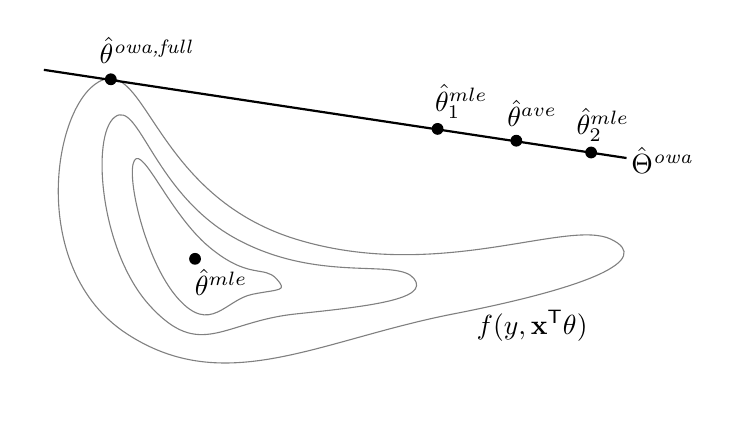
\begin{tikzpicture}
    [
    dot/.style = {minimum width=0.15cm,inner sep=0pt,line width=0pt,fill,circle,black,font=\small}
    ]
\draw[gray] plot [smooth cycle,tension=1] coordinates {(-0.5,-0.75) (-1.05,1) (-0.1,-0.1) (0.75,-0.5) (0.45,-0.7) };
\draw[gray] plot [smooth cycle,tension=1] coordinates {(-0.85,-0.85) (-1.3,1.55) (0.25,0) (2.5,-0.5) (1,-0.95)};
\draw[gray] plot [smooth cycle,tension=1] coordinates {(-1.15,-1.2) (-1.5,2) (1,0) (5,0) (3,-0.95)};

\draw[thick] (-2.2,2.15) -- (5.2,1.03);

\node[dot] (wstar) at (-0.28,-0.25) {};
\node at (0.05,-0.55) {$\wmle$};

%\node[dot] (wstarproj) at (0.1,1.8) {};
%\draw (wstar) -- (wstarproj);
%\draw (0.07,1.65) -- (0.23,1.62) -- (0.26,1.78);

%\node[dot] (wavestar) at (4,0.5) {};
%\node                 at (4.5,0.3) {$\E\wave$};
\node[dot] (wave) at (3.8,1.25) {};
\node at (4.0,1.6) {$\wave$};
\node[dot] (wave) at (2.80,1.40) {};
\node at (3.1,1.75) {$\wmle_1$};
\node[dot] (wave) at (4.75,1.10) {};
\node at (4.9,1.45) {$\wmle_2$};
%\node[dot] (wave) at (3.8,1.25) {};

\node[dot] at (-1.35,2.03) {};
\node at (-0.9,2.4) {$\wowafull$};

\node at (4,-1.1) {$f(y,\trans\x\w)$};
\node at (5.65,1.0) {$\W$};

\end{tikzpicture}
\caption{
    Our method performs a second round of optimization to find the best parameter vector in $\W$.
    Since $\wave\in\W$, the estimator $\wowafull$ has higher empirical likelihood than $\wave$ almost surely.
}
\label{fig:contour}
\end{figure}

\begin{algorithm}[t]
\caption{Estimation in two rounds}
\label{alg:distributed}
\begin{algorithmic}
\State Each machine $i$ independently
\State ~~~~~loads dataset $Z_i$
\State ~~~~~calculates $\wmle_i$
\State All machines broadcast $\wmle_i$ to all other machines
\State Each machine $i$ independently
\State ~~~~~constructs $\hat W$
\State ~~~~~randomly selects a dataset $Z^{reopt}_i\subset Z_i$
\State ~~~~~calculates $\Zproj_i=\{(\trans\x\hat W,y) : (\x,y)\in\Zreopt\}$
\State All machines broadcast $\Zproj_i$ to a master machine
\State The master calculates $\wowa$
\end{algorithmic}
\label{fig:alg2}
\end{algorithm}

%\begin{algorithm}[t]
%\caption{Estimation with common data}
%\label{alg:distributed}
%\begin{algorithmic}
%\State Each machine $i$ independently
%\State ~~~~~loads dataset $Z_i$
%\State ~~~~~calculates $\wmle_i$
%\State All machines broadcast $\wmle_i$ to all other machines
%\State Each machine $i$ independently
%\State ~~~~~constructs $\hat W$
%\State ~~~~~randomly selects a dataset $Z^{reopt}_i\subset Z_i$
%\State ~~~~~calculates $\trans\x\hat W$
%\State All machines broadcast $Z^{reopt}_i$ to a master machine
%\State The master calculates $\wowa$
%\end{algorithmic}
%%\label{fig:alg}
%\end{algorithm}

\section{RELATED WORK}

Related work can be divided into two categories:
alternative $q$ estimators,
and bounds on the communication complexity of distributed learning.

\subsection{Alternative estimators}
\label{sec:alt}
The simplest and most popular communication-efficient estimator is the averaging estimator
\begin{equation}
\wave = \frac{1}{m}\sum_{i=1}^m \wmle_i
\end{equation}

Previous analysis of $\wave$ makes a number of limiting assumptions.
\cite{mcdonald2009efficient} gave the first analysis of this estimator in the special case of L2 regularized maximum entropy models.
They provide tail bounds on $\ltwo{\wstar-\wave}$, showing that the variance of the estimator reduces as $O((nm)^{-1/2})$ with high probability,
but they could not show a reduction in bias.
Their analysis uses a martingale technique that requires the radius of the dataset be independent of the size of the dataset.
This is a particularly limiting assumption as even the simple case of Gaussian distributed data does not satisfy it.
\cite{zhang2012communication} provide a more general analysis showing that the Mean Squared Error (MSE) $\E\ltwo{\wstar-\wave}^2$ decays as $O((nm)^{-1} + n^{-2})$.
This matches the optimal MSE of $\wmle$ whenever $m<n$.
Their analysis still requires a number of technical assumptions.
For example, they assume the parameter space $\Theta$ is bounded.
This assumption does not hold under the standard Bayesian interpretation of L2 regularization as a Gaussian prior of the parameter space.
They further make strong convexity and 8\emph{th} order smoothness assumptions which guarantee that $\wmle_i$ is a ``nearly unbiased estimator'' of $\wstar$.
(As we will see in the next section,
recently developed information theoretic bounds show these assumptions are required to show a reduction in MSE to the single machine rate.)
Surprisingly, \cite{zhang2013divide} showed that in the special case of kernel ridge regression, a reduction in bias was not needed to have the MSE decay at the optimal sequential rate.
By a careful choice of regularization parameter, they caused $\wmle_i$ to have lower bias but higher variance, so that the final estimate of $\wave$ had both reduced bias and variance.

Other research has focused on modifications to the $\wave$ estimator to reduce bias.
\cite{zinkevich2010parallelized} showed that if the training sets partially overlap each other (instead of being disjoint), then the resulting estimator will have lower bias.
The authors admit their analysis is ``highly technical.''
\cite{zhang2012communication} also provided a bootstrap average estimator,
which works as follows.
Let $r\in(0,1)$, and $X_i^r$ be a bootstrap sample of $X_i$ with $rn$ data points.
Then the bootstrap average estimator is
\begin{equation}
\begin{aligned}
\wmler_i &= \argmax_\w \sum_{\x\in X_i^r} f(x;\w)
\\
\waver &= \frac{1}{m}\sum_{i=1}^m \wmler_i
\\
\wboot & = \frac{\wave-r\waver}{1-r}
\end{aligned}
\end{equation}
The intuition behind this estimator is to use the bootstrap sample to directly estimate and correct for the bias.
This estimator enjoys a MSE decaying as $O((nm)^{-1}+n^{-3})$.

%An alternative definition of the $\wave$ estimator is
%\begin{equation}
%\wave = \argmin_\w \frac{1}{m}\sum_{i=1}^m \ltwo{\wmle_i-\w}^2
%\end{equation}
%It is easy to show that the two definitions are equivalent with standard calculus.

\cite{liu2014distributed} propose a more Bayesian approach inspired by \cite{merugu2003privacy}.
Instead of averaging the model's parameters,
they directly ``average the models'' with the following KL-average estimator.
\begin{equation}
\wkl = \argmin_\w \sum_{i=1}^m \kl[\bigg]{p(\cdot;\wmle_i)}{p(\cdot;\w)}
\end{equation}
The minimization is performed via a bootstrap sample from the smaller models.
This method has two main advantages.
First, it is robust to reparameterizations of the model.
Second, it is statistically optimal for the class of non-interactive optimization methods.
(We show in the next section that their bound does not apply to our $\wowa$ estimator due to our semi-interactive setting.)
The main downside of the KL-average is that the minimization has a prohibitively high computational cost.
Let $n^{kl}$ be the size of the bootstrap sample.
Then the original implementation's MSE shrinks as $O((nm)^{-1}+(nn^{kl})^{-1})$.
This implies that the bootstrap procedure requires as many samples as the original problem to get a MSE that shrinks at the same rate as the averaging estimator.
\cite{han2016bootstrap} show a method to reduce this rate to $O((nm)^{-1}+(n^2n^{kl})^{-1})$ using control variates, but the procedure remains prohibitively expensive.
Their experiments show the procedure scaling only to datasets of size $nm\approx10^4$,
whereas our experiments involve a dataset of size $nm\approx10^8$

\subsection{Performance bounds}
\label{sec:bounds}

Performance bounds come in two flavors: statistical and information theoretic.
On the statistical side, \cite{liu2014distributed} showed that for an arbitrary function $q$ \emph{which does not depend on the data},
$\ltwo{\wq-\wmle}^2$ decays as $\Omega(\gamma^2_\wstar \I^{-1}_\wstar/n^2)$.
Here $\gamma_\wstar$ is the statistical curvature of the model and $\I_\wstar$ is the Fisher information.
Furthermore, they show that $\wkl$ matches this bound.
This bound is not relevant for our estimator because our merge function depends on the data.
Furthermore, we directly optimize $\ltwo{\wq-\wstar}^2$ which is a more useful quantity in practice.

\cite{shamir2014fundamental}, \cite{zhang2013information}, and \cite{garg2014communication} all provide information theoretic lower bounds on the sample complexity of non-interactive learning problems.
As above, however, there results are not applicable in our semi-interactive setting.
%provides general information theoretic bounds for what he terms learning with information constraints.
%As a special case of Shamir's analysis is the non-interactive communication model where $q$ does not depend on the data.
%When $q$ is allowed to depend on the data, his model no longer applies.
There is one information theoretic lower bound that does apply to us.
Let the true parameter vector $\wstar$ be $k$-sparse.
That is, $\lzero{\wstar} \le k$.
%Then \cite{zhang2013information} showed that at least $\Omega(mk/\log m)$ bits of communication are required in the non-interactive setting,
%and \cite{garg2014communication} improved this lower bound to $\Omega(mk)$.
Surprisingly, \cite{braverman2015communication} showed that the minimax optimal error rate for least squares regression requires $\Omega(m\cdot\min\{n,d\})$ bits of communication even in the fully interactive setting.
This is important because sparsity does not reduce the amount of communication required, and this bound does apply in our setting.

\section{ANALYSIS}
\label{sec:anal}

In this section, we analyze OWA's statistical performance.
The main tool we use is the Central Limit Theorem (CLT).
Informally, this theorem states that the $\wmle_i$ parameter vectors are approximately normally distributed.
%We then use results from the random projection literature to bound the distance
We then combine this result with standard results in random projections.
Classical versions of the CLT apply only in the limit as $n\to\infty$.
But we use a more advanced version of the CLT due to \cite{spokoiny2012parametricestimation} that applies in the finite sample case.
This approach makes our analysis simpler and more general than the analysis of algorithms discussed in Section \ref{sec:anal}.
All the technical details are handled by the CLT.
In particular, we prove novel bounds for the $\wave$ estimator.

We provide a simple bound that shows that averaging does not improve the bias of our estimator,
but reduces the variance at the rate $O((nm)^{-1})$.
Similar bounds are well known (see Section \ref{sec:alt}).
Our analysis has the following advantages:
it requires fewer assumptions, has a simpler proof, and has an easy to interpret constant factor.
The main idea of our technique is to show that the variance is normally distributed.
The ideas in this proof will be used in Section \ref{sec:analreopt} where we show that the variance of $\wowa$ is the same as $\wave$, but that the bias is reduced.
\begin{theorem}
Let $t>0$.
Then with probability at least $1-\exp(-t)$,
\begin{equation}
\ltwo{\wstar-\wave} \le \ltwo{\wstar-\E\wmle_i} + \sqrt\frac{v_t}{mn}
\end{equation}
where
\begin{equation}
v_t =
\tr{\I^{-1}_{\wtave}}
+ 2\sqrt{\tr \left({\I^{-2}_{\wtave}}\right)t}
+ 2\ltwo{\I^{-1}_{\wtave}}t
\end{equation}
\end{theorem}

\subsection {Non-Asymptotic Central Limit Theorem}

The standard central limit theorem for maximum likelihood estimation states that as the number of samples $n \to \infty$,
%the distribution of the parameter vector approaches a Gaussian at the rate $O(n^{-1/2}$).
\begin{equation}
\I^{-1/2}_\wstar(\w-\wstar) \to \frac{1}{\sqrt n}\normal{\zero}{I}
.
\end{equation}
See chapter 7 of \cite{lehmann1999elements} for an elementary presentation of this result.
In the non-asymptotic case, the distribution of the parameter vector is no longer Gaussian;
instead, it is subgaussian.
We say a random vector $\x$ with zero mean is \emph{subgaussian} with variance proxy $\sigma^2$ if
\begin{equation}
\prob{\ltwo{\x} > t} \le \exp(-\sigma^2 t^2 /2)
.
\end{equation}
In notation, we say
\begin{equation}
\x \sim \subnormal{\sigma^2}
.
\end{equation}
%We say that a random vector $\x\in\mathbb{R}^d$ is \emph{subgaussian} with variance proxy $\sigma>0$ if for all $\alpha\in\mathbb{R}^d$,
%\begin{equation}
%\E\exp(\trans\alpha\x) \le \exp(\ltwo{\alpha}^2\sigma^2/2)
%.
%\end{equation}
The simplest example of a subgaussian random variable is a multivariate normal vector with mean $\zero$ and covariance $I$.
In this case, $\sigma=1$.
See \cite{vershynin2010introduction} for a tutorial on subgaussian random variables,
including equivalent definitions and important results.

Before stating the theorem, we first state the theorem's three conditions.
The first condition is straightforward,
but next two conditions are more technical.
Despite the technical appearance of these assumptions,
they are highly general.
We note in particular that any generalized linear model (e.g. least squares, Poisson, and logistic regression),
and many models with nonconvex likelihood functions satisfy these conditions.
We include the conditions here for completeness,
but defer to \cite{spokoiny2012parametricestimation} for a more detailed discussion.

\begin{assumption}
The likelihood function $f(y,\trans\x\w)$ is two times differentiable with respect to $\w$.
\end{assumption}
\begin{assumption}
For all $u>0$, there exists a function $g_1(u)>0$ such that for all $|\lambda| \le g_1(u)$
and for all $\x\in\X$,
\begin{equation}
\sup_{\w:\ltwo{\I_\wstar(\w-\wstar)} \le u}
\log\E\exp\left(\lambda\frac{\trans\x\nabla_\w f(y_i,\trans\x\w)}{\ltwo{V\x}}\right)
\le
\frac{v_0^2\lambda^2}{2}
\end{equation}
where $\trans V V = \I_\wstar$ and $v_0$ is a constant.
\end{assumption}
\begin{assumption}
For all $u>0$, there exists a function $b(u)>0$ such that
\begin{equation}
\sup_{\w:\ltwo{\I_\wstar(\w-\wstar)} = u}
\log\E\exp\left(\frac{k(\w,\wstar)}{\ltwo{V(\w-\wstar)}}\right)
\le
b(u)
\end{equation}
where
$
k(\w,\wstar) = \E\left(f(y,\trans\x\w) - f(y,\trans\x\wstar)\right)
$
.
\end{assumption}

The following is a restatement of Theorem 5.2 in \cite{spokoiny2012parametricestimation}.
\begin{theorem}
Assume Conditions 1-3 hold.
Then whenever $t \le c\sqrt{p/n}$,
we have with probability at least
%Then with probability at least $1-\delta$,
%\begin{equation}
%\ltwo{V(\w-\wstar)} \le c\sqrt{\frac{d+\log{1/\delta}}{n}}
%\end{equation}
%where the constant $c$ depends on $v_o$, $g_1(u)$, and $b(u)$ defined above.
%Equivalently, we have that
%\begin{equation}
%V(\w-\wstar) \sim \subnormal{\sigma}
%\end{equation}
\end{theorem}

%%%%%%%%%%%%%%%%%%%%%%%%%%%%%%%%%%%%%%%%

\subsection {Proof of Theorem 1}

We have by the triangle inequality that
\begin{equation}
\ltwo{\wstar-\wave} \le \ltwo{\wstar-\E\wave} + \ltwo{\E\wave-\wave}
\label{eq:biasvar}
\end{equation}
The left term above captures the estimator's bias and the right term the variance.
First we consider the bias.
By the linearity of expectation, we have that
\begin{align}
\E\wave
&=
\E\frac{1}{m}\sum_{i=1}^m\wmle_i
%\\&=
=
\frac{1}{m}\sum_{i=1}^m\E\wmle_i
=
\E\wmle_i
\label{eq:expwave}
\end{align}
and so the bias term
$\ltwo{\wstar-\E\wave}
=
\ltwo{\wstar-\E\wmle_i}
$.
In words, the bias of the combined averaging estimator is the same as the bias of the estimator on an individual machine.

Now we consider the variance.
We have by Equations \ref{eq:expwave} and \ref{eq:assumption} that
\begin{align}
\wave-\E\wave
&=
%\frac{1}{m}\sum_{i=1}^m\wmle_i-\E\wave
%\\&=
\frac{1}{m}\sum_{i=1}^m\left(\wmle_i-\E\wave\right)
\label{eq:var1}
\\&=
\frac{1}{m}\sum_{i=1}^m\left(\wmle_i-\E\wmle_i\right)
\\&\sim
\frac{1}{m}\sum_{i=1}^m\left(\frac{1}{\sqrt n}\normal\zero{\I^{-1}_{\E\wave}}\right)
\\&=
\frac{1}{\sqrt {nm}}\normal\zero{\I^{-1}_{\E\wave}}
\label{eq:var2}
%\\&\sim
%\frac{1}{m}\normal{m\E\wmle_i}{\frac{m}{n}I^{-1}}
%\\&\sim
%\normal{\E\wmle_i}{\frac{1}{nm}I^{-1}}
%\\
%\wave-\E\wmle_i
%&\sim
%\normal{\zero}{\frac{1}{nm}I^{-1}}
%\\
%\wave-\E\wave
%&\sim
\end{align}
%Centering the distribution and applying Equation \ref{eq:expwave} gives
%\begin{equation}
%\E\wave-\wave
%\sim
%\normal{\zero}{\frac{1}{nm}I^{-1}}
%\end{equation}
In the last step we used the fact that adding a centered Gaussian to itself $m$ times is equivalent to multiplying the Gaussian by $\sqrt{m}$.
%So bounding the variance reduces to bounding the norm of a Gaussian.
Our last step is to bound the norm of the Gaussian in Equation \ref{eq:var2}.
Applying the bound in Proposition 1.1 from \cite{hsu2012tail} gives that with probability at least $1-\exp(-t)$,
\begin{equation}
\ltwo{\E\wave-\wave} \le \sqrt\frac{v_t}{nm}
\label{eq:ct1}
\end{equation}
%where
%\begin{equation}
%\begin{aligned}
%v_t'
   %= \tr\left({\frac{1}{mn}\I^{-1}_{\wtave}}\right)
%+ 2&\sqrt{\tr \left({\frac{1}{mn}\I^{-1}_{\wtave}}\right)^2t}&
%\\+ 2\ltwo{\frac{1}{nm}\I^{-1}_{\wtave}}t&
%\end{aligned}
%\end{equation}
%Then by the linearity of trace and scalability of norms,
%\begin{equation}
%v_t' =
%\frac{1}{mn}\left(
%\tr\I^{-1}_{\wtave}
%+ 2\sqrt{\tr \I^{-2}_{\wtave}t}
%+ 2\ltwo{\I^{-1}_{\wtave}}t
%\right)
%\label{eq:ct2}
%\end{equation}
Substituting Equations \ref{eq:expwave} and \ref{eq:ct1} into Equation \ref{eq:biasvar} gives the stated result.

Note that this reduction in variance is essentially optimal.
By an argument similar to Equations \ref{eq:var1}-\ref{eq:var2},
we can show that the variance of the maximum likelihood estimator trained on all of the data is
\begin{equation}
\wmle - \E\wmle \sim \frac{1}{\sqrt{mn}} \normal{\zero}{\I^{-1}_{\wmle}}
\label{eq:var3}
\end{equation}
The only difference between Equations \ref{eq:var2} and \ref{eq:var3} is the location of the Fisher information matrix.
%%%%%%%%%%%%%%%%%%%%%%%%%%%%%%%%%%%%%%%%

\subsection {Proof of Theorem 2}

Using the triangle inequality, we decompose $\ltwo{\wowa-\wstar}$ into three components:

\begin{equation}
\begin{aligned}
\ltwo{\wowa-\wstar}
&\le
\ltwo{\wowa-\wowastar}
\\&
+
\ltwo{\wowastar - \proj{\Wowa}\wstar}
\\&
+
\ltwo{\proj{\Wowa}\wstar - \wstar}
\end{aligned}
\end{equation}
The first term $\ltwo{\wowa-\wowastar}$ captures the approximation error due to the limited number of points in the second round of optimization.
The result follows by first bounding each of these terms individually,
then applying the union bound.

\subsubsection{Bounding the first term}

Our first lemma is a direct consequence of the central limit theorem.
%\begin{lemma}
%With probability at least $\delta$,
%\begin{equation}
%\ltwo{\wowa-\wowastar} \le
%\end{equation}
%\end{lemma}

\subsubsection{Bounding the second term}
The next lemma is a direct consequence of assumptions.

\subsubsection{Bounding the third term}
Then we have that with probability at least $(1-\exp(-t))^2$,
\begin{equation}
\ltwo{\wstar-\proj\W\wstar}
\le
%b_t\sqrt{\left(1-\frac{m}{d}\right)}
b_t\sqrt{\left(1-\frac{m}{d}\right)}
+
\sqrt\frac{v_{t}}{nm}
\end{equation}
where
%$\lzero{\wave} < d$ is the number of non-zero entries in the $\wave$ vector,
\begin{equation}
b_t = \frac{\lambda_{\min}}{\lambda_{\max}}\ltwo{\wstar-\E\wmle_i}\sqrt{t + 1}
\end{equation}
%with probability at least $1-\exp (-\frac{b}{2} (\tbias-\ln(\tbias+1)))$,
$\lambda_{\min}$ and $\lambda_{\max}$ are the minimum and maximum eigenvalues of $\I^{-1}_{\wave}$,
and $v_t$ is defined as in Theorem \ref{thm:wave}.


\subsection {Analyzing $\wowa$}

%We now extend the analysis of the previous section to the $\wowa$ estimator.
%We show that its variance is bounded by the variance of $\wave$,
%but that the bias shrinks as $O(1-m/d)$.
%
%Recall from Section \ref{sec:vcdim} that the estimator $\wowa$ has low error with high probability compared to any parameters in the space $\Wave$.
%Denote by $\proj\Wave$ the projection operator onto the space $\Wave$.
%In this section, we analyze the bias and variance of $\proj\Wave\wstar$.

%If $\A$ is an affine space, then denote by $\proj{\A}$ the projection operator onto $\A$.
We introduce the following notation.
If $\A$ is an arbitrary space,
then the projection of a point $\x$ onto $\A$ is denoted by
\begin{equation}
\proj{\A}\x = \argmin_{\mathbf{a}\in\A} \ltwo{\mathbf{a}-\x}
\end{equation}
Recall that $\W$ is the vector space spanned by the $\wmle_i$s.
In this section we analyze the estimator $\proj{\W}\wstar$.

\begin{theorem}
\label{thm:wave}
Let $t>0$.
Then we have that with probability at least $(1-\exp(-t))^2$,
\begin{equation}
\ltwo{\wstar-\proj\W\wstar}
\le
%b_t\sqrt{\left(1-\frac{m}{d}\right)}
b_t\sqrt{\left(1-\frac{m}{d}\right)}
+
\sqrt\frac{v_{t}}{nm}
\end{equation}
where
%$\lzero{\wave} < d$ is the number of non-zero entries in the $\wave$ vector,
\begin{equation}
b_t = \frac{\lambda_{\min}}{\lambda_{\max}}\ltwo{\wstar-\E\wmle_i}\sqrt{t + 1}
\end{equation}
%with probability at least $1-\exp (-\frac{b}{2} (\tbias-\ln(\tbias+1)))$,
$\lambda_{\min}$ and $\lambda_{\max}$ are the minimum and maximum eigenvalues of $\I^{-1}_{\wave}$,
and $v_t$ is defined as in Theorem \ref{thm:wave}.
\end{theorem}

\ignore{
\begin{theorem}
%Assume that $n$ is large enough that $\wmle_i$ is distributed according to $\normal{\wtave}{\I^{-1}_{\wtave}}$.
%Let $\delta\in(0,1)$.
%Then with probability at least $1-\delta$,
We have that
\begin{equation}
\ltwo{\wstar-\proj\Wave\wstar}
\le \epsilon_{bias} + \epsilon_{var}
\end{equation}
where for all $\tbias>0$,
\begin{equation*}
%\begin{split}
%\prob{
    \epsilon_{bias}
    \le
    \ltwo{\wstar-\wtave}\sqrt{(\tbias + 1)\left(1-\frac{m}{d}\right)}
%}
%\\
%\ge
%1-\exp \bigg(-\frac{b}{2} (\beta-\ln(\beta+1))\bigg)~~&
%\end{split}
\end{equation*}
with probability at least
$1-\exp (-\frac{b}{2} (\tbias-\ln(\tbias+1)))$
and for all $\tvar>0$,
\begin{equation*}
\begin{split}
&\epsilon_{var}
\\
&\le
\sqrt{
    \frac{1}{m}
    \left(\tr{\I^{-1}_{\wtave}}
        + 2\sqrt{\tr ({\I^{-2}_{\wtave}})\tvar}
        + 2\ltwo{\I^{-1}_{\wtave}}\tvar
    \right)
}
\end{split}
\end{equation*}
with probability at least $1-\exp(-\tvar)$.

%\begin{equation}
%\begin{split}
%&\ltwo{\wstar-\proj\Wave\wstar}
%\\
%&\le
%\ltwo{\wstar-\wtave}\sqrt{(\beta + 1)\left(1-\frac{m}{d}\right)}
%\\
%&+
%\sqrt{
    %\frac{1}{m}
    %\left(\tr{\I^{-1}_{\wtave}}
        %+ 2\sqrt{\tr ({\I^{-1}_{\wtave}}^2)t}
        %+ 2\ltwo{\I^{-1}_{\wtave}}t
    %\right)
%}
%\le
%\exp \bigg(-\frac{b}{2} (\beta-\ln(\beta+1))\bigg)~~&
%\end{split}
%\end{equation}
\end{theorem}
}

\begin{proof}
This proof follows the same form as the proof for Theorem \ref{thm:wave}.
We first decompose the error into a bias and variance component;
then we bound each component separately.
To decompose the error, we need to introduce the following affine space.
\begin{align}
\Waff&=\affspan \{\wmle_i\}_{i=1}^m
\\
\WaffE&=\affspan \{\wmle_i - \wave + \E\wave\}_{i=1}^m
\end{align}
We now have that
\begin{align}
\ltwo{\wstar-\proj\W\wstar}
&\le
\ltwo{\wstar-\proj\Waff\wstar}
\\
&\le
\ltwo{\wstar-\proj\WaffE\wstar}
%\\&
+
\ltwo{\proj\WaffE\wstar-\proj\Waff\wstar}
%\\&+
%\ltwo{\proj\Wtave\wstar-\proj\Wave\wstar}
\end{align}
The first line above follows because $\Waff\subseteq\W$,
and the second by the triangle inequality.
The left term of the inequality above can be thought of as akin to the bias of the estimator $\proj\Waff\wstar$,
and the right term can be thought of as akin to the variance.

We begin by bounding the right term.
We have that with probability at least $1-\exp(-t)$,
\begin{align}
&\ltwo{\proj\WaffE\wstar-\proj\Waff\wstar}
\\
&=
\ltwo{(\proj\Waff\wstar+\wave-\wtave)-\proj\Waff\wstar}
\\&=
\ltwo{\wave-\wtave}
\\&\le
\sqrt\frac{v_t}{mn}
\end{align}
The first equality follows because the space $\WaffE$ is a translation of $\Waff$ by the vector $(\wave-\wtave)$.
The probabilistic inequality is due to Equation \ref{eq:ct1} in the proof of Theorem \ref{thm:wave}.

We now bound the left term.
Define the vector space
\begin{equation}
\V=\vecspan \{\wmle_i - \wtave\}_{i=1}^m
\end{equation}
which is the translation of the affine space $\WaffE$ to include the origin.
Then we have that
%Note that $\proj\Wtave$ is not a linear projection but an affine projection.
%We first apply a translation so that we are working with the linear projection $\proj\W$.
\begin{align}
\ltwo{\wstar-\proj\WaffE\wstar}
&=
\ltwo{(\wstar-\wtave)-\proj\V(\wstar-\wtave)}
\\&=
\ltwo{(I-\proj\V)(\wstar-\wtave)}
\end{align}
In the first step, we translate the vectors so that the affine projection onto $\Wtave$ becomes a linear projection onto $\W$.
The operator $(I-\proj\W)$ is a random projection onto a $(d-m)$-dimensional space.

%Now, $(I-\proj\W)$ is a random projection onto a subspace of dimension $d-m$.
%(\fixme{This projection is not chosen uniformly at random because the covariance of $\wmle_i$ is not the identity.})
%This gives us that for all $\tbias>0$,
%\begin{equation}
%\begin{split}
%\prob{\ltwo{\wstar-\proj\Wtave\wstar} \ge \ltwo{\wstar-\wtave}\sqrt{(\tbias + 1)\left(1-\frac{m}{d}\right)}}&
%\\
%\le
%\exp \bigg(-\frac{b}{2} (\tbias-\ln(\tbias+1))\bigg)~~&
%\end{split}
%\end{equation}
\ignore{
Note that the space $\Wave$ depends on the data.
Therefore, we can think of $\proj\Wave\wstar$ as an estimator of $\wstar$.
As in the proof of Theorem \ref{thm:wave},
we begin by decomposing the MSE of $\proj\Wave\wstar$ into its bias and variance components.
\begin{equation}
\begin{split}
\ltwo{\wstar-\proj\Wave\wstar}^2
&=
\ltwo{\wstar-\E\proj\Wave\wstar}^2
\\&+
\ltwo{\E\proj\Wave\wstar-\proj\Wave\wstar}^2
\end{split}
\end{equation}
We begin with the variance.

%Define $\Wtave = \vecspan\{\wmle_i-\wtave\}_{i=1}^m$.
%Then,
We have that
\begin{align}
\ltwo{\wstar-\proj\Wave\wstar}
&\le
\ltwo{\wstar-\proj\Wtave\wstar}
+
\ltwo{\proj\Wtave\wstar-\proj\Wave\wstar}
\\
&=
\ltwo{\wstar-\proj\Wtave\wstar}
+
\ltwo{\wave-\wtave}
\label{eq:errdecomp}
\end{align}
The first line follows from the triangle inequality.
The second line follows because every point in $\Wtave$ is a translation of a point in $\Wave$ by the vector $\wave-\wtave$.

Define the spaces
\begin{align}
\W&=\vecspan\{\wmle_i - \wave\}_{i=1}^m\\
\Wave&=\affspan\{\wave_i\}_{i=1}^m\cup\{\wave\}\\
\Wtave&=\affspan\{\wave_i\}_{=1}^m\cup\{\wtave\}
%\Wave&=\vecspan\{\wave_i-\wave\}_{i=1}^m\\
%\Wtave&=\vecspan\{\wave_i-\wtave\}_{i=1}^m
\end{align}
Denote by $\proj\A$ to be the projection operator onto the space $\A$.
Denote by $\I_\w$ the Fischer information matrix at the point $\w$.

%\begin{lemma}
%Let $a$ and $b$ be integers with $b<a$.
%Let $\x$ be a random vector on the $a$ dimensional unit sphere.
%Let $T : \mathbb{R}^a \to \mathbb{R}^b$ be the projection operator that preserves the first $b$ coordinates of a vector and drops the rest.
%Then for all $\beta>0$,
%\begin{equation}
%\prob{\ltwo{T\x} \ge \sqrt{(\beta + 1)\frac{b}{a}}}
%\le
%\exp \left(\frac{b}{2}(-\beta+\ln(\beta+1))\right)
%\end{equation}
%\end{lemma}

We will now bound the two terms in Equation \ref{eq:errdecomp} separately.
To bound the left term, we introduce the following lemma.
It is adapted from Lemma 2.2 in \cite{dasgupta2003elementary}.
It has been simplified to ignore cases irrelevant for our purpose.
\begin{lemma}
Let $a$ and $b$ be integers with $b<a$.
Let $\x\in\mathbb{R}^a$ be an arbitrary vector.
Let $T : \mathbb{R}^a \to \mathbb{R}^b$ be projection onto a subspace of size $b$ distributed uniformly at random.
Then for all $\beta>0$,
\begin{equation}
\begin{split}
\prob{\ltwo{T\x} \ge \ltwo\x\sqrt{(\beta + 1)\frac{b}{a}}}&
\\
\le
\exp \bigg(-\frac{b}{2} & (\beta-\ln(\beta+1))\bigg)
\end{split}
\end{equation}
\end{lemma}
To apply this lemma, note that $\proj\Wtave$ is not a linear projection but an affine projection.
We first apply a translation so that we are working with the linear projection $\proj\W$.
\begin{align}
\ltwo{\wstar-\proj\Wtave\wstar}
&=
\ltwo{(\wstar-\wtave)-\proj\W(\wstar-\wtave)}
\\
&=
\ltwo{(I-\proj\W)(\wstar-\wtave)}
\end{align}
Now, $(I-\proj\W)$ is a random projection onto a subspace of dimension $d-m$.
(\fixme{This projection is not chosen uniformly at random because the covariance of $\wmle_i$ is not the identity.})
This gives us that for all $\tbias>0$,
\begin{equation}
\begin{split}
\prob{\ltwo{\wstar-\proj\Wtave\wstar} \ge \ltwo{\wstar-\wtave}\sqrt{(\tbias + 1)\left(1-\frac{m}{d}\right)}}&
\\
\le
\exp \bigg(-\frac{b}{2} (\tbias-\ln(\tbias+1))\bigg)~~&
\end{split}
\end{equation}
}

\end{proof}

%The following lemma is adapted from Theorem 3.1 in \cite{matouvsek2008variants}.
%It has been simplified to ignore cases irrelevant for our purpose.
%\begin{lemma}
%Let $a$ and $b$ be integers with $a>b$.
%Let $T\in\mathbb{R}^{a\times b}$ be a random matrix with entries drawn i.i.d. from the standard normal distribution.
%Let $\x\in\mathbb{R}^a$ be an arbitrary vector.
%Then there exists a constant $c$ such that for all $\delta\in(0,1)$,
%\begin{equation*}
%\prob{\ltwo{T\x} \le \left(\sqrt{b}+c\sqrt{\log\frac{\delta}{2}}\right)\ltwo\x} \le 1-\delta
%\end{equation*}
%\end{lemma}

%\begin{cor}
%%Assume that Conditions (1-5) hold.
%%Then as $n\to\infty$,
%%\begin{enumerate}
%%\item
%If $f$ is locally $\sigma$-strongly convex,
%\begin{equation}
%\ltwo{\wstar-\wowa} \le
%\end{equation}
%%\end{enumerate}
%\end{cor}
%
%\begin{proof}
%\end{proof}

%\subsection{Proposed Solution}
%
%We propose the following solution.
%Define the matrix $W : \mathbb{R}^{d\times m}$ to have $i$th column equal $\wmle_i$.
%%That is,
%%\begin{equation}
%%W = (\wmle_1, \wmle_2, ..., \wmle_m)
%%\end{equation}
%Then our estimator is defined as
%\begin{equation}
%\begin{aligned}
%\alpha &= \argmax_\w \sum _{(\x,y)\in Z_i} f(y,\trans\x W\w)
%\\
%\w &= \trans W \alpha
%\end{aligned}
%\end{equation}
%Note that the inner $\w$ above is a vector of dimension $m$, not $d$ (as elsewhere).
%In words
%%In words, this estimator takes the dataset $Z'$ and projects it onto the subspace spanned by the

\newpage

\clearpage

\newpage
\ignore{
\section{ANALYSIS}

First we justify why only a small number of data points is needed for the second optimization.
For simplicity, we'll restrict our discussion to the case of binary classification.
This lets us use standard VC-dimension arguments.

\subsection{Few datapoints are needed in the optimization}

%Recall the following theorem from standard VC theory.
%\begin{theorem}
%Let $Z$ be a dataset of $n$ points sampled i.i.d. from distribution $\D$.
%Let $\wmle$ be the parameters of the maximum likelihood estimator of $Z$.
%Let $L : \Theta \to \mathbb{R}$ be the true 0-1 loss on the distribution $\D$.
%Let $d$ be the VC dimension of the hypothesis class $\Theta$.
%Then with probability at least $1-\delta$,
%\begin{equation}
%L(\wmle) \le L(\wstar) + O\left(\sqrt{\frac{d + \log(1/\delta)}{n}}\right)
%\end{equation}
%\end{theorem}
%For an extended discussion of the above theorem,
%see for example Chapter 6 of \cite{shalev2014understanding}.
\begin{theorem}
%Let $\Y=\{0,1\}$.
Define $\alpha^{*}$ to be the optimal parameter constrained to the space spanned by the columns of $W$.
In notation,
\begin{equation}
\alpha^{*} = \argmax_{\alpha} \int_{\Y\times\X} f(y,\trans\x W\alpha) d(y,\x)
\end{equation}
Define $L : \mathbb{R} \to \mathbb{R}$ to be the 0-1 loss over the true data distribution.
Then with probability at least $1-\delta$,
\begin{equation}
L(\alpha^*) \le L(\alpha) + O\left(\sqrt{\frac{m + \log(1/\delta)}{n^{reopt}}}\right)
\end{equation}
\end{theorem}
\begin{proof}
For each machine $i$, fix the set of data points $Z_i$
(which in turn fixes the $\wmle_i$).
Define $\A$ to be the space of parameters
\begin{equation}
\A=\{\trans W\w : \w \in \Theta\}
\end{equation}
The linear hypothesis class defined by $\A$ has VC dimension $m$.
Since each of the data points in $Z^{reopt}$ is independent of $W$,
the result follows immediately from standard VC theory.
See for example Chapter 6 of \cite{shalev2014understanding}.
\end{proof}

\begin{theorem}

\end{theorem}

\ignore{
\subsection{Overall growth}

In this section we assume the following regularity conditions.

\begin{theorem}
Assume conditions (1-5) above hold.
%Let $m$ be arbitrary.
Then in the limit as $n$ approaches $\infty$:
\begin{enumerate}
\item
If $f$ is locally $\sigma$-strongly convex around $\wstar$
\begin{equation}
\Pr{a}
\end{equation}
\item
If $f$ is locally $\ell$-Lipschitz around $\wstar$
(i.e. ),
then
\begin{equation}
\end{equation}
\end{enumerate}
\end{theorem}

\begin{lemma}
\label{lem:normaff}
Let $W : \mathbb{R}^{d\times m}$ be a random matrix where each entry is distributed as a standard Gaussian.
Let $\Wave$ be the affine hull of the columns of $W$;
that is,
\begin{equation}
\Wave = \left\{\sum_{i=1}^m c_i\wmle_i : c\in\mathbb{R}, \sum_{i=1}^m c_i = 1 \right\}
\end{equation}
Then for all $t$,
\begin{equation}
\Pr\left[\ltwo{\proj{W}0}^2 > O(t(1-m/d))\right] \le 1 - \exp(-t)
\end{equation}
\end{lemma}
}
}

\section{EXPERIMENTS}
\label{sec:exp}

We test our parallelization procedure on two logistic regression tasks.
The first task uses synthetic data.
The second task uses real world add click data from the tencent search engine.

\subsection{Synthetic Data}

\begin{figure*}[t]
%\begin{tikzpicture}
\begin{tabular}{ccc}
  \includegraphics[width=0.3\textwidth]{img/logl2-auto-logl2-auto-normal-log-1000-100-star.pdf}
& \includegraphics[width=0.3\textwidth]{img/logl2-auto-logl2-auto-normal-log-1000-1000-star.pdf}
& \includegraphics[width=0.3\textwidth]{img/logl2-auto-logl2-auto-normal-log-1000-10000-star.pdf}
\\
  \includegraphics[width=0.3\textwidth]{img/logl2-auto-logl2-auto-uniform-log-1000-100-star.pdf}
& \includegraphics[width=0.3\textwidth]{img/logl2-auto-logl2-auto-uniform-log-1000-1000-star.pdf}
& \includegraphics[width=0.3\textwidth]{img/logl2-auto-logl2-auto-uniform-log-1000-10000-star.pdf}
\\
  \includegraphics[width=0.3\textwidth]{img/logl1-auto-logl2-auto-laplace-log-1000-100-star.pdf}
& \includegraphics[width=0.3\textwidth]{img/logl1-auto-logl2-auto-laplace-log-1000-1000-star.pdf}
& \includegraphics[width=0.3\textwidth]{img/logl1-auto-logl2-auto-laplace-log-1000-10000-star.pdf}
\\
  \includegraphics[width=0.3\textwidth]{img/logl1-auto-logl2-auto-spike-log-1000-100-star.pdf}
& \includegraphics[width=0.3\textwidth]{img/logl1-auto-logl2-auto-spike-log-1000-1000-star.pdf}
& \includegraphics[width=0.3\textwidth]{img/logl1-auto-logl2-auto-spike-log-1000-10000-star.pdf}
\end{tabular}
%\end{tikzpicture}
\caption{}
\end{figure*}

\begin{figure}
%\begin{tikzpicture}
\begin{tabular}{c}
\\ \includegraphics[width=0.45\textwidth]{img/logl2-star-logl2-auto-normal-log-1000-100-100.pdf}
%\\ \includegraphics[width=0.45\textwidth]{img/logl2-star-logl2-auto-uniform-log-1000-100-100.pdf}
\\ \includegraphics[width=0.45\textwidth]{img/logl1-star-logl2-auto-laplace-log-1000-100-100.pdf}
\\ \includegraphics[width=0.45\textwidth]{img/logl1-star-logl2-auto-spike-log-1000-100-100.pdf}
%\\ \includegraphics[width=0.45\textwidth]{img/logl2-star-logl2-auto-normal-log-1000-1000-100.pdf}
%\\ \includegraphics[width=0.45\textwidth]{img/logl2-star-logl2-auto-normal-1000-100-100.pdf}
\end{tabular}
%\end{tikzpicture}
\caption{
    A similar effect happens when $d=1000$ or $d=10000$,
    but it is much less pronounced.
}
\end{figure}

We consider two logistic regression models.
In the first,
each component of the parameter vector $\theta_i$ is sampled i.i.d. from the standard normal distribution.
This is the Bayesian interpretation of $L2$ regularization.
In the second, $\theta_i$ is sampled i.i.d. from the Laplace (two-sided exponential) distribution with scale 1.
This is the Bayesian interpretation of $L1$ regularization.
In both models, the data points are then sampled as
\begin{equation}
\begin{aligned}
%\theta &\sim \normal{0}{I}
%\\
\x_i &\sim \normal{0}{I}
,
~~~
%y_i &= \frac{1}{1+\exp(-\trans\x_i\theta)}
y_i = \left(1+\exp(-\trans\x_i\theta)\right)^{-1}
\end{aligned}
\end{equation}

Our first experiment shows how the parallel algorithms scale as the number of machines $m$ increases.
We fix $n=1000$ data points per machine, so the size of the dataset $mn$ grows as we add more machines.
This simulates the typical ``big data'' scenario where data is abundant,
but processing resources are scarce.
We further consider three regimes:
%high dimensional ($d=10000$), medium dimensional ($d=1000$), and low dimensional ($d=100$) data.
more data than dimensions ($d=100$),
one data point per dimension ($d=1000$),
and less data than dimensions ($d=10000$).

%The advantage of artificial data is that we know the true model parameters and can evaluate our estimators' performance using the mean squared error.
%We test against two GLMs: an ordinary least squares regression and a logistic regression.
%In both experiments, we pick a constant dimension $d$ and a constant number of data points per machine $n$, then vary the number of machines $m$.
%In total, there are $mn$ data points for each trial.
%Each trial is repeated 100 times, and the reported results are the average.
%
%To evaluate the performance of our parallelization procedure, we evaluate against 4 baseline estimators.
%The first (Naive) is the performance of just a single machine on $n$ data points without merging the results.
%The second (Oracle) is the performance using all $mn$ data points on a single machine.
%For large values of $n$ or $m$ this would of course be impractical to calculate.
%The third (Ave) is the average of all the parameter vectors from each machine.
%The fourth (BootstrapAve) is evaluated according to the following procedure.
%Each machine $i$ calculates a parameter estimate $\theta_i$ using all the $n$ data points it has available,
%and a second estimate $\theta_i'$ using only $rn$ data points (where $r$ is a constant between 0 and 1).
%The final estimator is given by:
%
%$$
%\frac{\theta_i - r\theta_i'}{1-r}
%$$
%
%The idea of this procedure is to estimate the bias of the model using the smaller sample, and return a bias corrected estimate of the final procedure.
%In practice, the value of the $r$ parameter greatly affects the estimator's performance, and this parameter must be set by cross-validation.
%In our experiments, we use each of the values in the set $\{0.5,0.4,0.3,0.2,0.1,0.05,0.02,0.01,0.05\}$ and report only the best possible $r$ value.
%Our method has no similar parameters to tune, and tends to perform better than BootstrapAve even when the latter uses the optimal $r$ parameter.
%
%\subsubsection{Data from an ordinary leasts squares model}
%The true model parameters $\theta$ were generated according to one of three priors:
%the uniform distribution over $[0,1]$,
%the standard normal distribution,
%and the standard laplace distribution.
%Our data set $X$ was then generated from a standard normal distribution,
%and the corresponding $Y$ values sampled from $X^T\theta + h(X,\theta) + \epsilon$,
%where $\epsilon$ is the standard normal distribution.
%We use three different values of $h$ to evaluate the effect of incorrect modeling assumptions on our estimators.
%The function $h(X,\theta)=0$ tests the case when our model assumptions are correct.
%In this case, the OLS estimator is unbiased.
%%The function $h(X,\theta)=

\subsection{Real World Advertising Data}

\section{CONCLUSION}

%%%%%%%%%%%%%%%%%%%%%%%%%%%%%%%%%%%%%%%%%%%%%%%%%%%%%%%%%%%%%%%%%%%%%%%%%%%%%%%%

\bibliographystyle{plainnat}
\bibliography{paper}

%%%%%%%%%%%%%%%%%%%%%%%%%%%%%%%%%%%%%%%%%%%%%%%%%%%%%%%%%%%%%%%%%%%%%%%%%%%%%%%%

\newpage
\section*{Appendix: Detailed Central Limit Theorem}

\begin{theorem}
Assume () and ().
If for all $u_0 > 0$,
\begin{align}
n^{1/2}u_0b & \ge 6 v_0 \sqrt{x+cp}
\label{eq:cond1}
\\
1 + \sqrt{x+cp} &\le 3b^{-1}v_0^2g_1(u_0) n^{1/2}
\label{eq:cond2}
\end{align}
then
\begin{equation}
\prob{\ltwo{\vv_0(\w-\wstar)} > u_0} \le \exp(-x)
.
\end{equation}
\end{theorem}

Manipulating Equation \ref{eq:cond1} gives
\begin{align}
\end{align}

\end{document}
